\documentclass[tikz,border=2]{standalone}
\newcommand{\leadblock}{C^{\mathrm{lead}}}
\newcommand{\trailblock}{C^{\mathrm{trail}}}
\newcommand{\mD}{\mathcal{D}}
\usetikzlibrary{decorations.pathreplacing,shadows,arrows,shapes,positioning,calc,backgrounds,fit}
% Define the layers to draw the diagram
%
\begin{document}
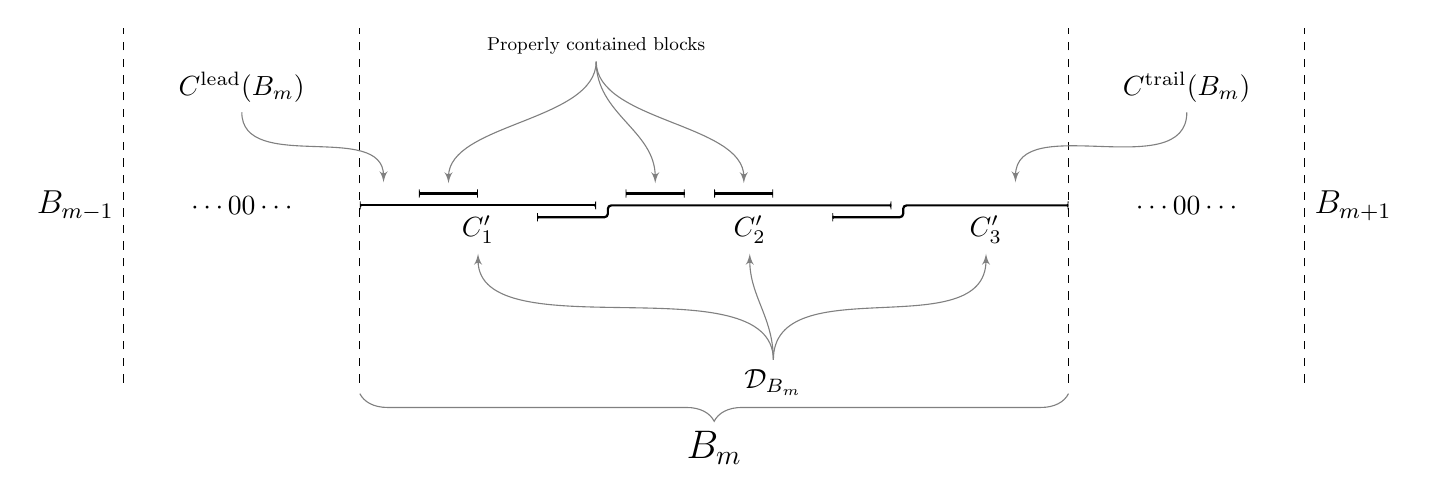
\begin{tikzpicture}
[node distance=1cm,scale=1.5,
block/.style={thick,>=serif cm,rounded corners=1.24pt},
vertex/.style={shape=circle,draw=black,inner sep=2pt},
dedge/.style={gray,>=latex', shorten >=.0pt, shorten <=.0pt},
myedge/.style={thick}]
% band boundaries
\draw[dashed] (2,-1.5) -- (2,1.5) node[midway,left] {\large $B_{m-1}$};
\draw[dashed] (4,-1.5) -- (4,1.5); % node[midway,left] {$B_{m-1}$};
\draw[dashed] (10,-1.5) -- (10,1.5); % node[left] {\Large $B_{m}$};
\draw[dashed] (12,-1.5) -- (12,1.5) node[midway,right] {\large $B_{m+1}$};
\node at (3,0) {$\cdots 00\cdots$};
\node at (11,0) {$\cdots 00\cdots$};

% D_B
\draw[block,<->] (4,0) -- (6,0) node[midway,below] (c1) {$C'_1$};
\node[] (lead) at (3,1) {$\leadblock(B_m)$};
\draw[dedge,->] (lead) edge[out=-90,in=90] ($(c1)+(-.8,.4)$);
\draw[block,<->] (5.5,-.1) -- (6.1,-.1) -- (6.1,0) -- (8.5,0) node[midway,below] (c2) {$C'_2$};
\draw[block,<->] (8,-.1) -- (8.6,-.1) -- (8.6,0) -- (10,0) node[midway,below] (c3) {$C'_3$};
\node[] (trail) at (11,1) {$\trailblock(B_m)$};
\draw[dedge,->] (trail) edge[out=-90,in=90]  ($(c3)+(.25,0.4)$);
\node (DB) at (7.5,-1.5) {$\mD_{B_m}$};
\draw[dedge,<-] (c1) edge[out=-90,in=90,looseness=.8] (DB);
\draw[dedge,<-] (c2) edge[out=-90,in=90,looseness=1] (DB);
\draw[dedge,<-] (c3) edge[out=-90,in=90,looseness=1] (DB);

\draw [gray,decorate,decoration={brace,amplitude=10pt,mirror,raise=4pt},yshift=0pt]
(4,-1.5) -- (10,-1.5) node [midway,below,yshift=-.5cm,black] {\Large $B_m$};

% properly contained blocks
\draw[block,<->] (4.5,.1) -- (5,.1) node[midway] (p1) {};
\draw[block,<->] (6.25,.1) -- (6.75,.1) node[midway] (p2) {};
\draw[block,<->] (7,.1) -- (7.5,.1) node[midway] (p3) {};
\node[scale=.75] (prop) at (6,1.35) {\small Properly contained blocks};
\draw[dedge,<-] (p1) edge[out=90,in=-90,looseness=.8] (prop);
\draw[dedge,<-] (p2) edge[out=90,in=-90,looseness=1] (prop);
\draw[dedge,<-] (p3) edge[out=90,in=-90,looseness=.8] (prop);
\end{tikzpicture}
{}
\end{document}
